% !TeX root=../main.tex
\chapter{نتایج}
%\thispagestyle{empty} 
\section{مقدمه} 
پس از پایان فرایند آزمون در دو حالت فشرده‌سازی منفرد و دسته‌ای و به‌دست‌آوردن مقادیر صرفه‌جویی زمانی، توان مصرفی و سربار زمانی، نتایج ذیل نمودارهایی گزارش خواهد شد. به منظور بصری‌سازی هرچه‌بهتر نمودار هر کدام از پارامترهای اندازه‌گیری به صورت منفک به نمایش درآمده‌است. هم‌چنین برای دریافت یک دید کلی از میزان هر کدام از سربارهای یادشده در یک نمودار نرمال‌شده حجم صرفه‌جویی‌شده در کنار این سربارها به نمایش در‌آمده‌اند. این فرآیند برای هرکدام از دو حالت بلوک‌های منفرد و دسته‌ای تکرار شده‌است.

\section{نتایج به‌دست‌آمده}
\subsection{فشرده‌سازی در حالت منفرد}


با توجه به نتایج به‌دست‌آمده، نمودار فضای صرفه‌جویی‌شده ذیل چهار پیاده‌سازی مختلف در
\ref{fig:sep-space}
 قابل‌مشاهده است.
\begin{figure}[ht]
	\centerline{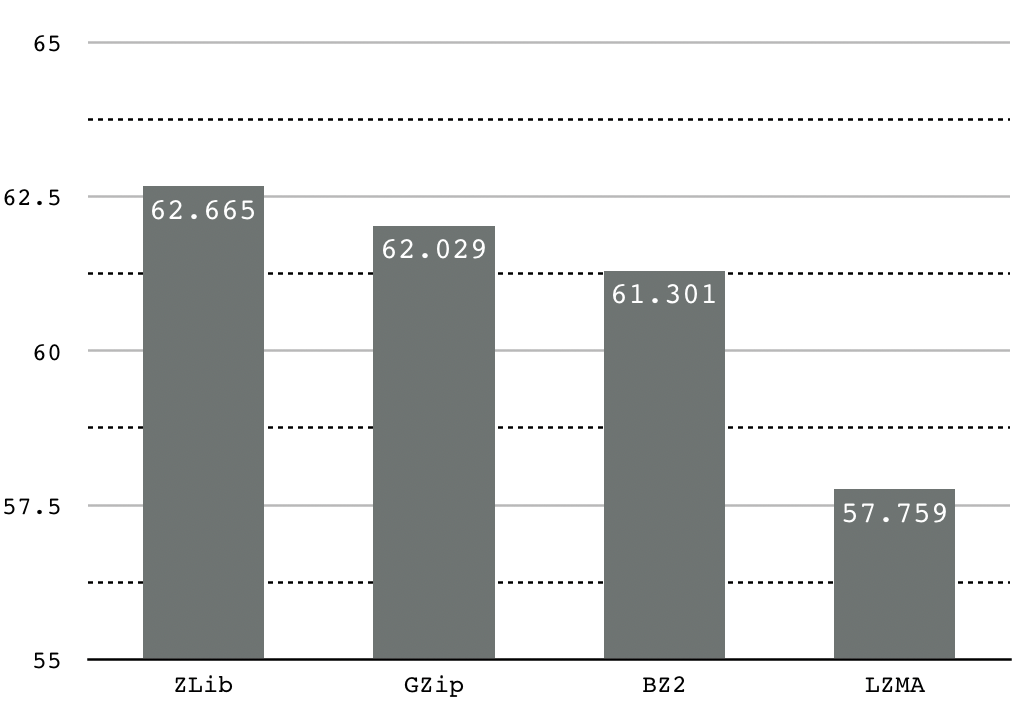
\includegraphics[width=0.5\textwidth]{sep-space.png}}
	\caption{نمودار فضای صرفه‌جویی}
	\label{fig:sep-space}
\end{figure}\\

نتایج آزمون بر اساس پارامتر سربار زمان ذیل چهار پیاده‌سازی مختلف در شکل
\ref{fig:sep-time}
 قابل‌مشاهده است.
\begin{figure}[ht]
	\centerline{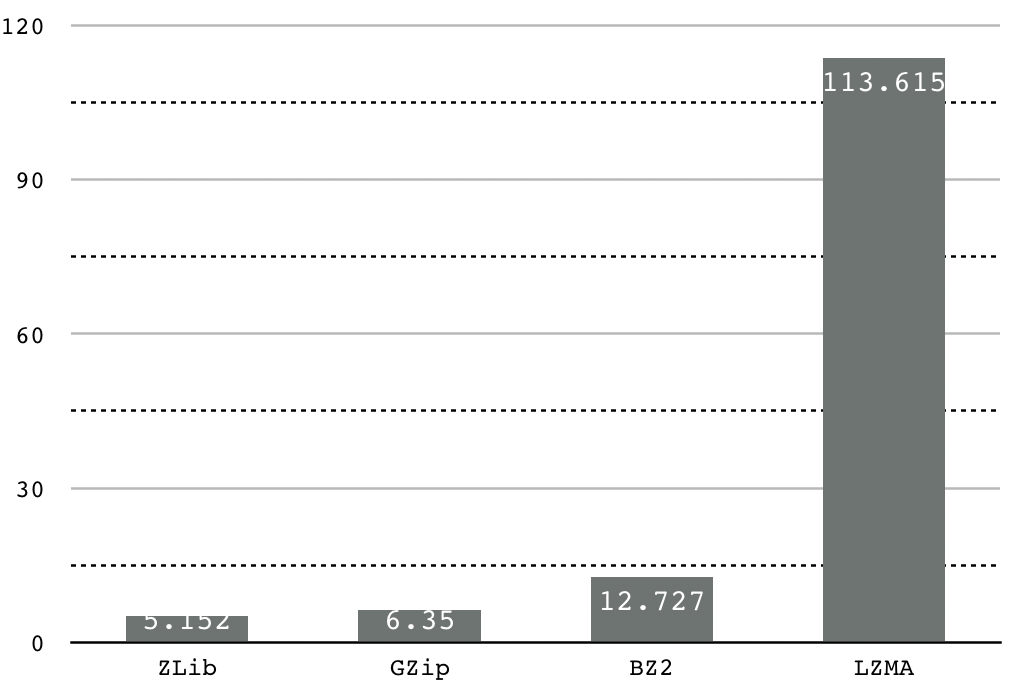
\includegraphics[width=0.5\textwidth]{sep-time.png}}
	\caption{نمودار سربار زمانی}
	\label{fig:sep-time}
\end{figure}\\

مقدار توان مصرفی به عنوان پارامتر مورد بحث ذیل چهار پیاده‌سازی مختلف در شکل
\ref{fig:sep-power}
 قابل‌مشاهده است.
\begin{figure}[ht]
	\centerline{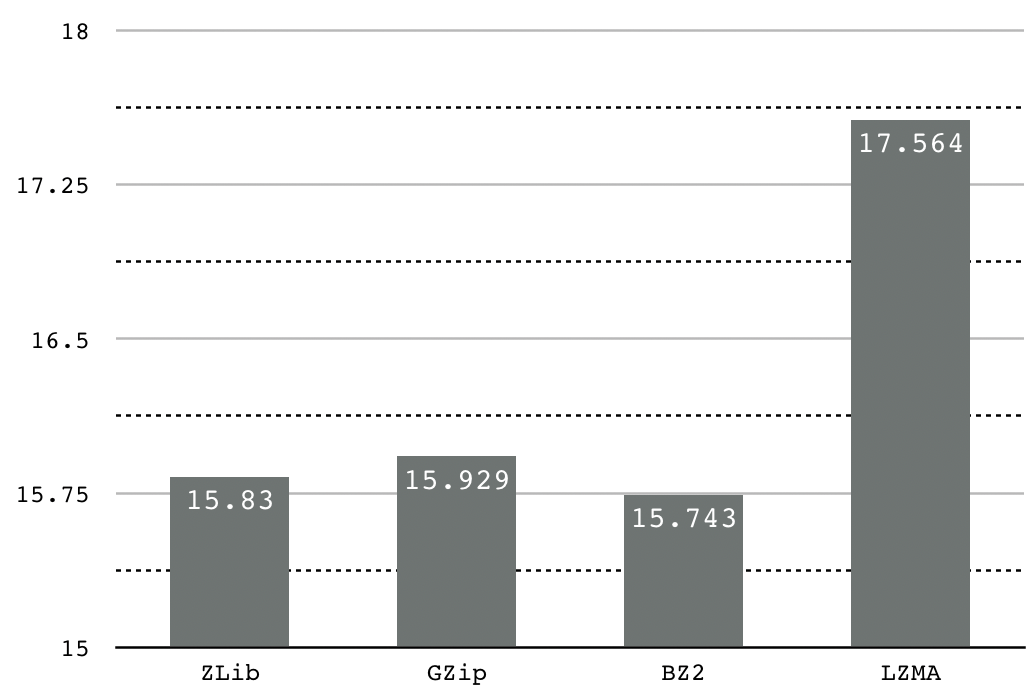
\includegraphics[width=0.5\textwidth]{sep-power.png}}
	\caption{نمودار توان مصرفی}
	\label{fig:sep-power}
\end{figure}\\

\subsection{فشرده‌سازی در حالت دسته‌ای}


نمودار فضای صرفه‌جویی‌شده برای چهار پیاده‌سازی انجام‌شده در
\ref{fig:chunk-space}
نشان داده شده‌است.
\begin{figure}[ht]
	\centerline{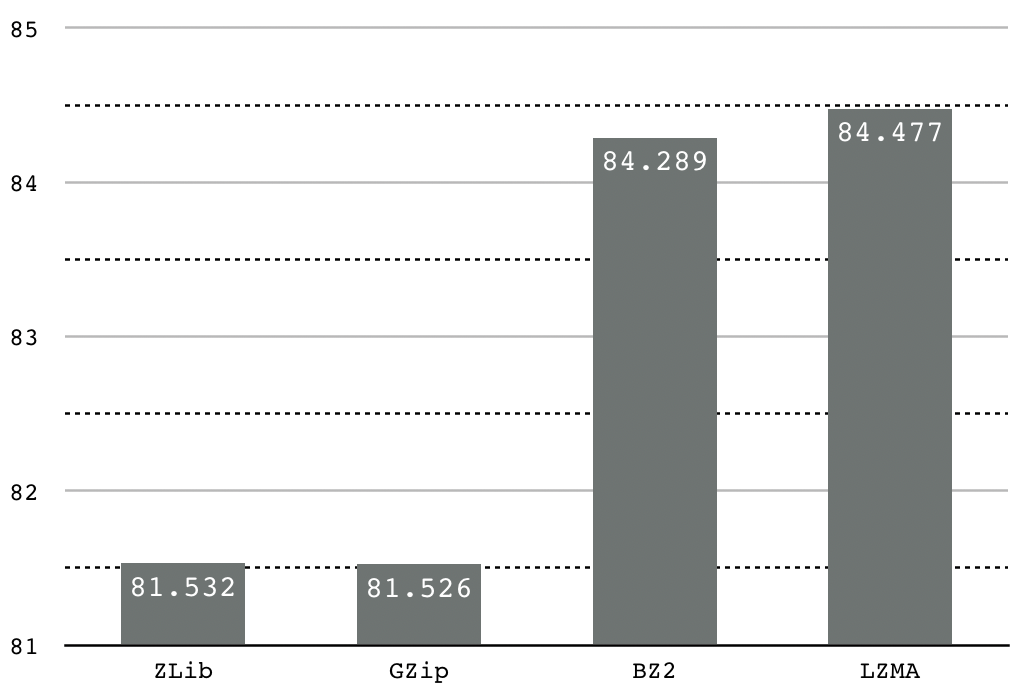
\includegraphics[width=0.5\textwidth]{chunk-space.png}}
	\caption{نمودار فضای صرفه‌جویی}
	\label{fig:chunk-space}
\end{figure}\\

نتایج به‌دست‌آمده برای پارامتر سربار زمان ذیل چهار پیاده‌سازی مختلف در شکل
\ref{fig:chunk-time}
دیده می‌شود.
\begin{figure}[ht]
	\centerline{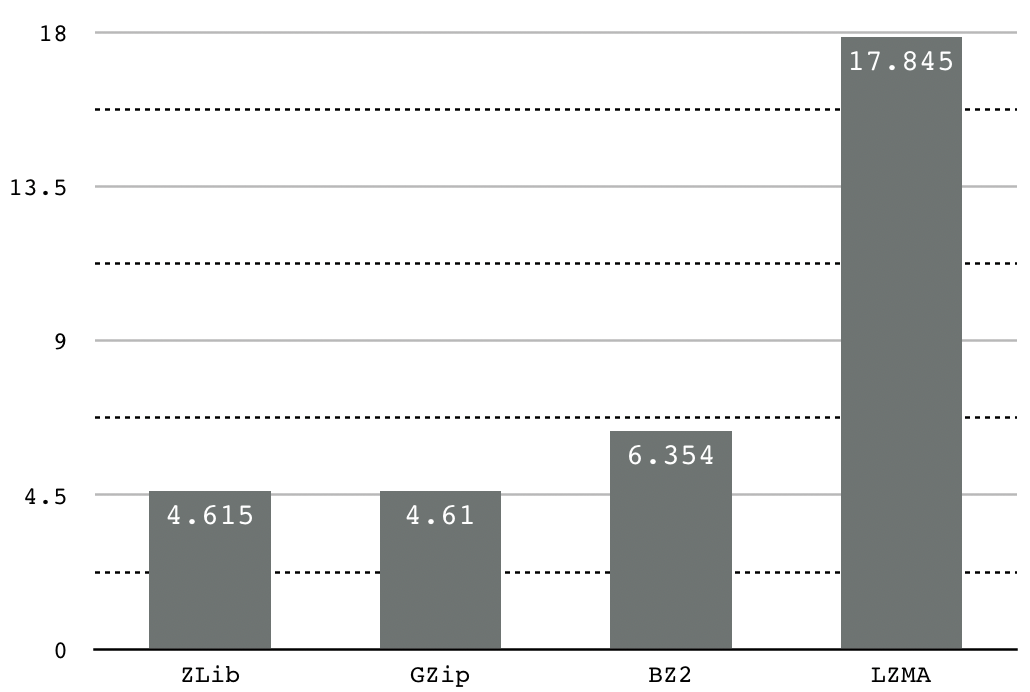
\includegraphics[width=0.5\textwidth]{chunk-time.png}}
	\caption{نمودار سربار زمانی}
	\label{fig:chunk-time}
\end{figure}\\

با درنظرگرفتن توان مصرفی به عنوان پارامتر مورد بحث در چهار پیاده‌سازی درنظرگرفته‌شده در شکل
\ref{fig:chunk-power}
قابل‌مشاهده است.
\begin{figure}[ht]
	\centerline{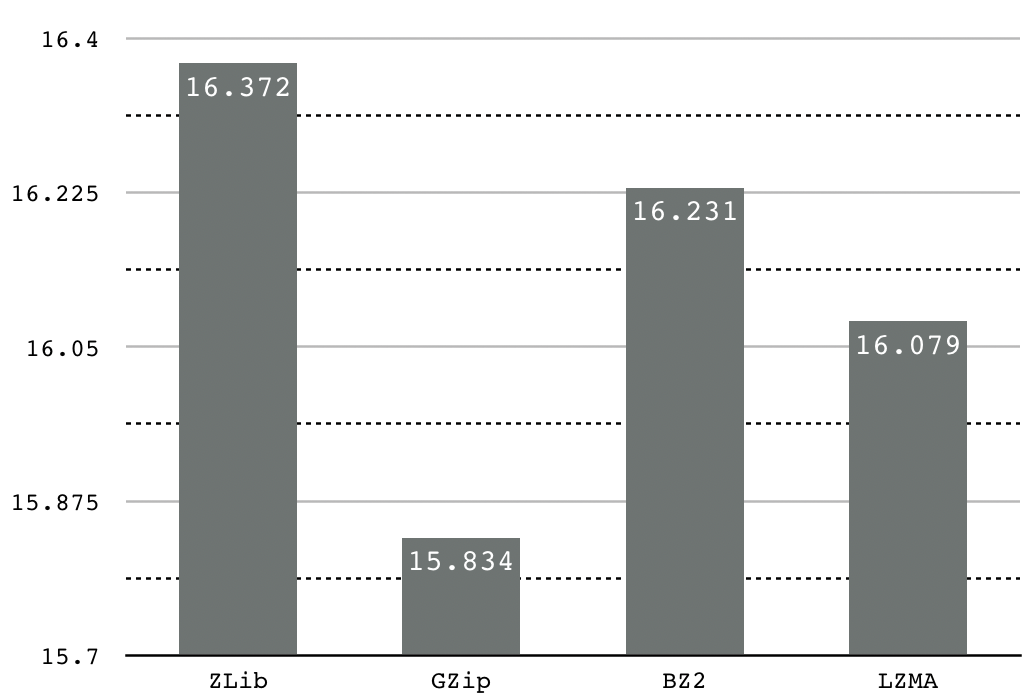
\includegraphics[width=0.5\textwidth]{chunk-power.png}}
	\caption{ نمودار توان مصرفی در حالت فشرده‌سازی دسته‌ای}
	\label{fig:chunk-power}
\end{figure}\\



\section{تحلیل نتایج}

پیاده‌سازی در دو حالت منفرد و دسته‌ای انجام و ذیل هرکدام از این آزمایش‌ها الگوریتم‌های مختلف فشرده‌سازی به کار گرفته شد. برای هرکدام از روش‌های استفاده‌شده، پارامترهای میزان فضای صرفه‌جویی‌شده،‌سربار زمانی و توان مصرفی ارزیابی شده‌است. با توجه به نتایج به‌دست‌آمده و نمودارهای متناظر می‌توان بین فشرده‌سازی‌های مختلف مقایسه انجام داد. 

با توجه به نتایج به‌دست‌آمده، همان‌طور که قبل از اجرای آزمون‌های متعدد با روش‌های فشرده‌سازی متفاوت پیش‌بینی می‌شد، حالت فشرده‌سازی دسته‌ای به مراتب میزان فضای صرفه‌جویی‌شده‌ی بیشتری را در اختیار ما قرار می‌داد. دلیل این امر آن است که آنتروپی با افزایش احتمال رخ‌دادن یک پیشامد کاهش می‌یابد و ذیل فشرده‌سازی دسته‌ای مقدار آنتروپی به حد چشم‌گیری کاهش می‌یابد. تأثیر این کاهش به حدی ا‌ست که بهترین حالت فشرده‌سازی دسته‌ای در مقایسه با بهترین حالت فشرده‌سازی منفرد بیشتر از ۲۰٪ بهبود را نشان می‌دهد.

از میان آزمایش‌های انجام‌شده بهترین الگوریتم فشرده‌سازی در هر دوحالت منفرد و دسته‌ای از منظر میزان فضای صرفه‌جویی‌شده به ترتیب ZLib و LZMA هستند. نکته‌ی حائز اهمیت در این‌جا آن است که الگوریتم LZMA در حالت فشرده‌سازی منفرد بدترین عملکرد را در میان الگوریتم‌های فشرده‌سازی بررسی‌شده دارد. این در حالی است که الگوریتم ZLib در حالت دسته‌ای نیز عملکرد قابل‌قبولی از خود به نمایش می‌گذارد. 

با بررسی توان مصرفی هرکدام از الگوریتم‌های فشرده‌سازی منتخب،‌ نتیجه می‌شود در حالت دسته‌ای الگوریتم ZLib بیشترین توان مصرفی و الگوریتم GZip کمترین توان مصرفی را موجب می‌شود. نکته‌ی شایان ذکر در این‌جا آن است که تفاوت میزان توان مصرفی این دو الگوریتم تفاوت معنادار و علمی با یکدیگر ندارد و می‌توان با تقریب خوبی این دو الگوریتم را از حیث میزان توان مصرفی برابر در نظر گرفت. درست است که توان مصرفی GZip از بین الگوریتم‌های بررسی‌شده کمترین مقدار را به خود اختصاص داده‌است اما از آن‌جایی که میزان فضای صرفه‌جویی‌شده توسط الگوریتم LZMA در حالت دسته‌ای بیشتر است و هم‌چنین توان مصرفی آن تفاوت قابل‌توجهی با GZip ندارد، می‌توان نتیجه گرفت که LZMA با در کنار هم قرار دادن توان مصرفی و میزان فضای صرفه‌جویی‌شده عملکرد بهتری دارد.

هم‌چنین در حالت فشرده‌سازی منفرد با توجه به نتایج به‌دست‌آمده مشاهده می‌شود که الگوریتم LZMA با اختلاف توان مصرفی بیشتری را در مقایسه با سایر الگوریتم‌های فشرده‌سازی صرف می‌کند. سایر الگوریتم‌های فشرده‌سازی  مورد آزمایش را می‌توان در یک مرتبه خواند. با در نظر گرفتن این موضوع، می‌توان استدلال نمود که الگوریتم فشرده‌سازی با میزان فضای صرفه‌جویی‌شده‌ی بیشتر، نسبت به سایر الگوریتم‌های فشرده‌سازی هم‌مرتبه از نظر توان مصرفی، اولویت دارد. در ادامه با توجه به برتری الگوریتم ZLib در مقایسه با الگوریتم LZMA از حیث میزان فضای صرفه‌جویی‌شده در حالت فشرده‌سازی منفرد و توان مصرفی کمتر الگوریتم ZLib می‌توان نتیجه گرفت که الگوریتم ZLib در حالت فشرده‌سازی منفرد برتری دارد.

\section{جمع‌بندی}

